\documentclass[a4paper]{article}
%\VignetteIndexEntry{Plotting Haplotype Networks}
%\VignettePackage{pegas}
\usepackage[utf8]{inputenc}
\usepackage{fancyvrb}
\usepackage{color}

\newcommand{\code}{\texttt}
\newcommand{\loci}{\code{"loci"}}
\newcommand{\NA}{\code{NA}}
\newcommand{\pkg}{\textsf}
\newcommand{\ape}{\pkg{ape}}
\newcommand{\pegas}{\pkg{pegas}}

\author{Emmanuel Paradis}
\title{Plotting Haplotype Networks with \pegas}

\usepackage{Sweave}
\begin{document}

\maketitle
\tableofcontents

\vspace{1cm}

\setkeys{Gin}{width=\textwidth}

\section{Background}

\subsection{Layout Algorithm}

\begin{Schunk}
\begin{Sinput}
R> data(woodmouse)
R> d <- dist.dna(woodmouse, "N")
R> nt <- rmst(d, quiet = TRUE)
\end{Sinput}
\end{Schunk}

\section{New Features in \pegas\ 1.0}

\subsection{Improved ``Replotting''}

\subsection{Haplotype Symbol Shapes}

The area of a disc is $\pi r^2$ with $r$ being the radius of the disc, so if
we want the area of the symbols to be proportional to \code{size}, we
should square-root them. However, in practice this masks differences
if most values in \code{size} are not very different (see
below). Instead, the diameters of the symbols ($2r$) are equal to the
values in \code{size}. If these are very heterogeneous, they could be
transformed with \code{size = sqrt(...} keeping in mind that the legend
will be on this new scale.

\begin{Schunk}
\begin{Sinput}
R> par(xpd = TRUE)
R> size <- c(1, 3, 5, 10)
R> x <- c(0, 5, 10, 20)
R> plot(0, 0, type="n", xlim=c(-2, 30), asp=1, bty="n", ann=FALSE)
R> other.args <- list(y = -5, inches = FALSE, add = TRUE,
+                    bg = rgb(1, 1, 0, .3))
R> o <- mapply(symbols, x = x, circles = sqrt(size / pi),
+             MoreArgs = other.args)
R> other.args$y <- 5
R> o <- mapply(symbols, x = x, circles = size / 2,
+             MoreArgs = other.args)
R> text(x, -1, paste("size =", size), font = 2, col = "blue")
R> text(30, -5, expression("circles = "*sqrt(size / pi)))
R> text(30, 5, "circles = size / 2")
\end{Sinput}
\end{Schunk}
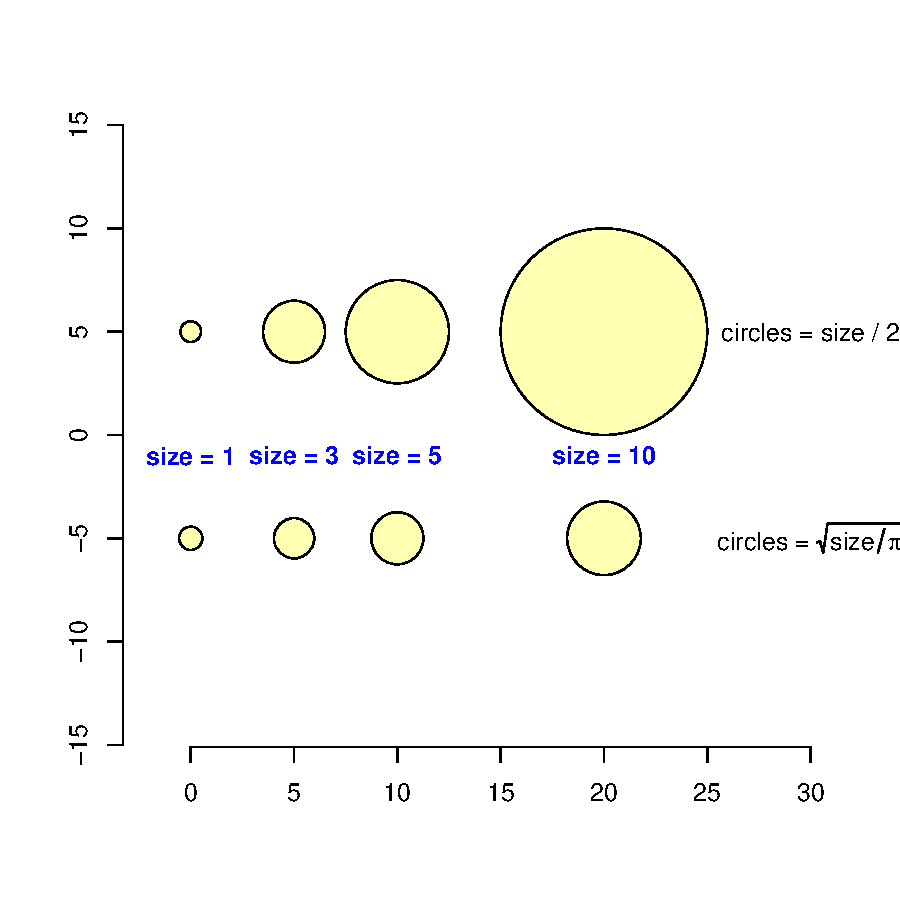
\includegraphics{PlotHaploNet-003}

\noindent For squares and diamonds, their areas are equal to the discs for the
same values given to \code{size}:

\begin{Schunk}
\begin{Sinput}
R> x <- c(0, 6, 13, 25)
R> plot(0, 0, type="n", xlim=c(-2, 30), asp=1, bty="n", ann=FALSE)
R> other.args$y <- 0
R> o <- mapply(symbols, x = x, circles = size/2, MoreArgs = other.args)
R> other.args$col <- "black"
R> other.args$add <- other.args$inches <- NULL
R> o <- mapply(pegas:::square, x = x, size = size, MoreArgs = other.args)
R> o <- mapply(pegas:::diamond, x = x, size = size, MoreArgs = other.args)
R> text(x, -7, paste("size =", size), font = 2, col = "blue")
\end{Sinput}
\end{Schunk}
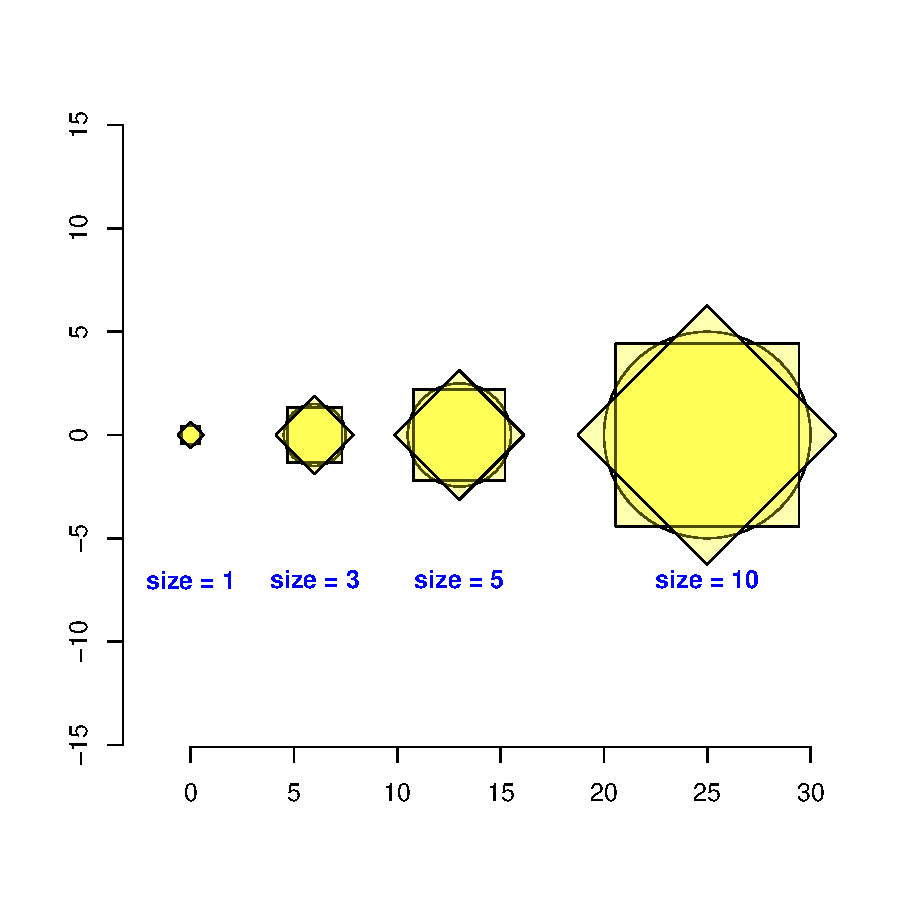
\includegraphics{PlotHaploNet-004}

\noindent A diamond is simply a square rotated 45\textdegree\ around its center.

\subsection{Themes}


\begin{Schunk}
\begin{Sinput}
R> plot(nt)
\end{Sinput}
\end{Schunk}
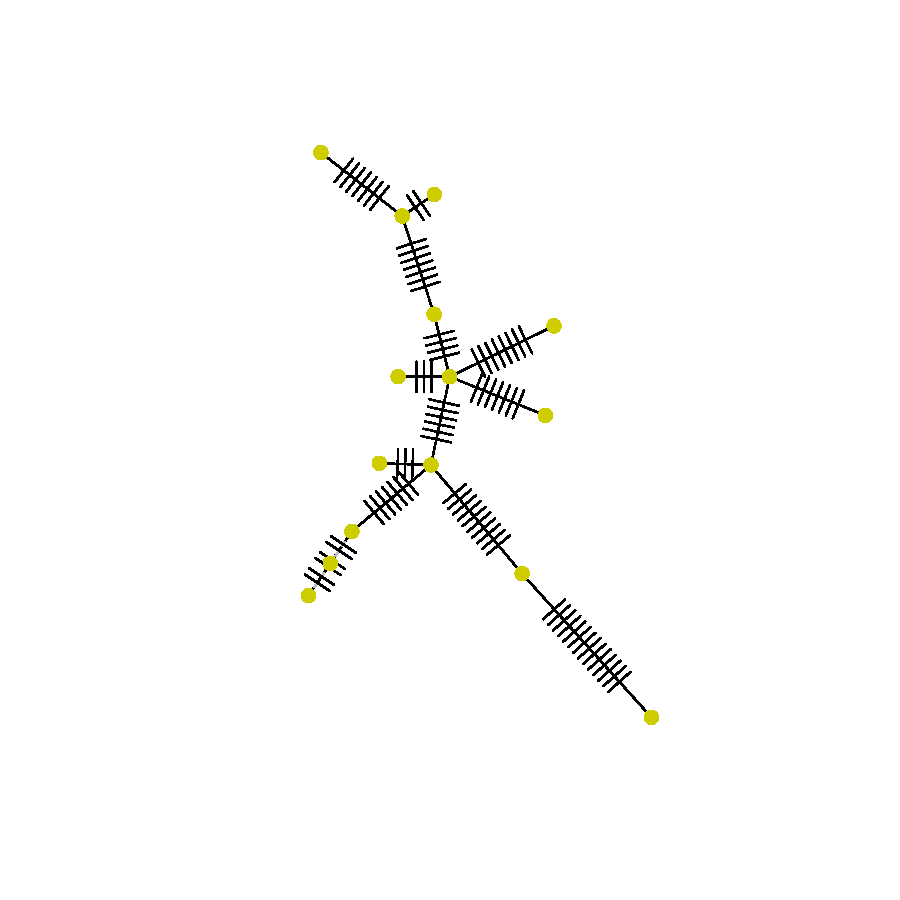
\includegraphics{PlotHaploNet-005}


\begin{Schunk}
\begin{Sinput}
R> setHaploNetTheme("puma")
R> plot(nt)
\end{Sinput}
\end{Schunk}
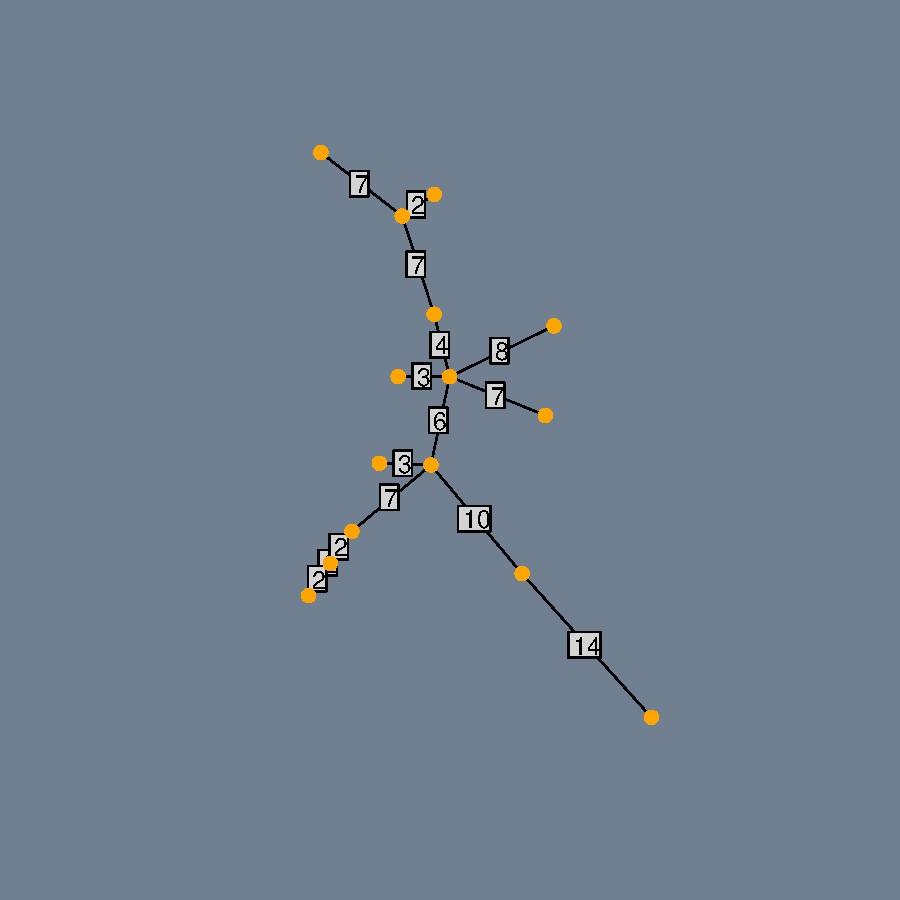
\includegraphics{PlotHaploNet-006}

\begin{Schunk}
\begin{Sinput}
R> setHaploNetTheme("tiger")
R> plot(nt)
\end{Sinput}
\end{Schunk}
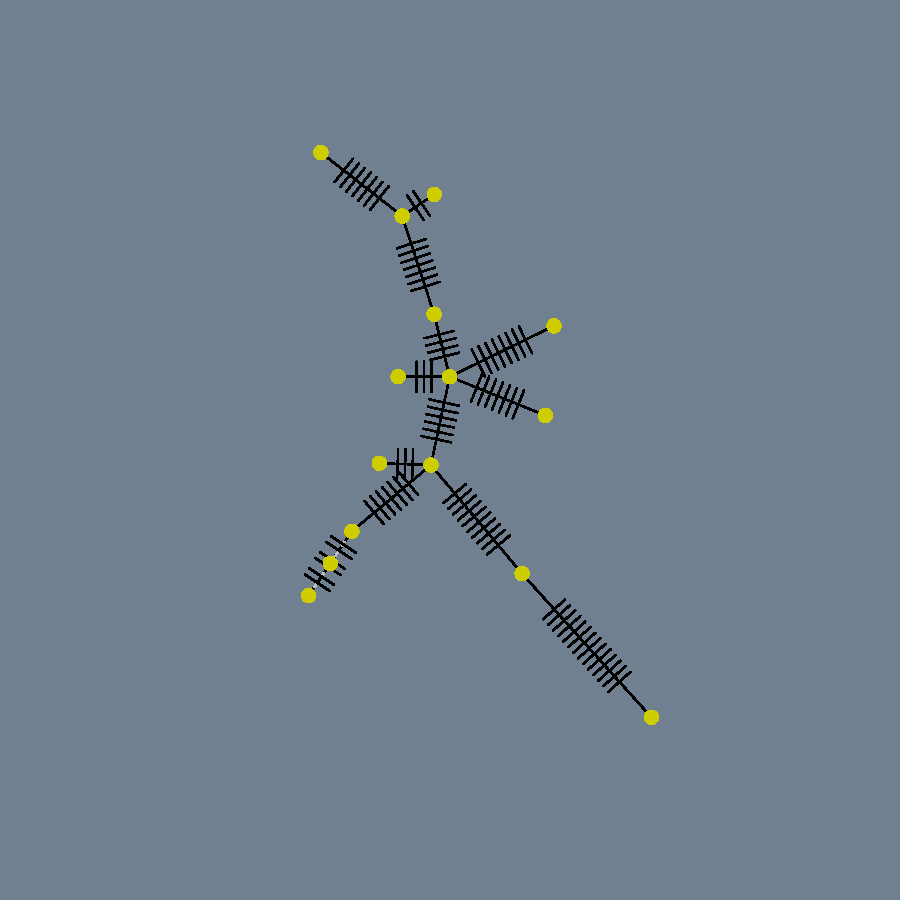
\includegraphics{PlotHaploNet-007}

\end{document}

